%*************************************************
% A template for PhD and MSc thesis. V1.0.
% Please see "guideline.pdf" first.
%*************************************************
% Iman Izadi, 1394
% Dept. of Electrical and Computer Engineering, IUT
%*************************************************
% این قالب بر اساس "شیوه‌نامه تدوین پایان‌نامه‌ها و رساله‌های 
%تحصیلات تکمیلی" دانشگاه صنعتی اصفهان تهیه شده است
%*************************************************

\documentclass[a4paper,fleqn]{report} 
%\usepackage{refcheck}


\usepackage{listings}
\usepackage{color}

\definecolor{dkgreen}{rgb}{0,0.6,0}
\definecolor{gray}{rgb}{0.5,0.5,0.5}
\definecolor{mauve}{rgb}{0.58,0,0.82}

\lstset{frame=tb,
	language=C,
	aboveskip=3mm,
	belowskip=3mm,
	showstringspaces=false,
	columns=flexible,
	basicstyle={\small\ttfamily},
	numbers=none,
	numberstyle=\tiny\color{gray},
	keywordstyle=\color{blue},
	commentstyle=\color{dkgreen},
	stringstyle=\color{mauve},
	breaklines=true,
	breakatwhitespace=true,
	tabsize=3
}


% All the packages and general definitions are included in this file: preamble.tex
%*************************************************
% All the packages and definitions are included here.
%*************************************************
%*************************************************
% Iman Izadi, 1394
% Dept. of Electrical and Computer Engineering, IUT
%*************************************************

\usepackage{amsthm,amssymb,amsmath}			% Writing math
\usepackage{epsf,graphicx}									% Including graphics
\usepackage[a4paper]{geometry}							% Fixing page layout and margins
\usepackage{titlesec}											% Change chapter and section titles
\usepackage{setspace}											% Change line spacing
\usepackage[stable,bottom]{footmisc}					% Move footnotes to the bottom of page

\usepackage{zref-perpage}									% Reset footnote counter in each page
\zmakeperpage[1]{footnote}

\usepackage{xepersian}										% Persian
\settextfont{XB Zar}												% Persian font


% Use English digits in equations
\DefaultMathsDigits

% Default footnotes from left to right
\setfootnoteLR

% Use English numbers for English footnotes
\makeatletter
\def\@makeLTRfnmark{\hbox{\@textsuperscript{\latinfont\@thefnmark}}}
\renewcommand\@makefntext[1]{%
    \parindent 1em%
    \noindent
    \hb@xt@1.8em{\hss\if@RTL\@makefnmark\else\@makeLTRfnmark\fi}#1}
\makeatother

% Use dash instead of dot in section numbers
\SepMark{-}										

% Change fonts and margins of section and subsection titles
% For chapters please see firstpages.tex
\titlespacing*{\section}{0pt}{1cm}{0.2cm}
\titleformat{\section}
  {\fontsize{12}{6}\scshape\bfseries}{\thesection}{1em}{}

\titlespacing*{\subsection}{0pt}{.8cm}{0cm}
\titleformat{\subsection}
  {\fontsize{11}{6}\scshape\bfseries}{\thesubsection}{1em}{}
  
% Fix table of contents for chapters
\makeatletter 
\def\@chapter[#1]#2{\ifnum \c@secnumdepth >\m@ne
     \refstepcounter{chapter}%
     \typeout{\@chapapp\space\thechapter.}%
     \addcontentsline{toc}{chapter}%
       	{\@chapapp~\protect\numberline{\tartibi{chapter}\,:\space #1}}
  \else
  	 \addcontentsline{toc}{chapter}{#1}%
  \fi
  \chaptermark{#1}%
  \addtocontents{lof}{\protect\addvspace{10\p@}}%
  \addtocontents{lot}{\protect\addvspace{10\p@}}%
  \@makechapterhead{#2}%
  \@afterheading}
\makeatother
							



\begin{document}

% The first pages (before abstract) are included in this file: firstpages.tex
%*************************************************
% In this file the first few pages are typeset.
% Make the changes accordingly
%*************************************************

% شماره صفحات با حروف
\pagenumbering{adadi}

%***************************
% 1st page: Blank
%***************************
\thispagestyle{empty}
\mbox{}
\pagebreak

%***************************
% 2nd page: Besmelah
%***************************
\thispagestyle{empty}
\begin{center}
	~\vfill
	
\includegraphics[scale=1]{besm1.jpg}
	~\vfill
\end{center}
\pagebreak

%***************************
% 3rd page: Title
%***************************
\thispagestyle{empty}
%\pagenumbering{gobble}
\newgeometry{left=3cm,right=3cm,top=2cm}
\begin{center}

\includegraphics[height=3cm]{iut_logo.png}
\vspace{0.4cm}

\textbf{دانشگاه صنعتی اصفهان}\\
\vspace{0.4cm}

{\large

	دانشکده مهندسی برق و کامپیوتر
}
\vspace{3.5cm}

{\Large
	\textbf{تبدیل خودکار کد ﻣﻨﺒﻊ ﺳﯿﺴﺘﻢ ﻋﺎﻣﻞ از زبان C ﺑﻪ زبان مدلسازی  Promela جهت استفاده برای تست و ارزیابی خودکار مدل}\\
}
\vspace{3.5cm}

{\Large
	پروژه کارشناسی دانشکده کامپیوتر -- نرم افزار\\
}
\vspace{1cm}

{\large
	\textbf{مرضیه علیدادی}\\
}
\vspace{3.5cm}

{\large
	استاد راهنما\\
}
\vspace{0.5cm}

{\large
	\textbf{دکتر الهام محمودزاده}\\
}
\vspace{3.5cm}

\textbf{1400}

\end{center}
\restoregeometry
\pagebreak

%***************************
% 4th page: Signatures
%***************************


%***************************
% 5th page: Acknowledgment
%***************************


%***************************
% 6th page: Rights
%***************************


%***************************
% 7th page: Dedication
%***************************


%***************************
% 8th page: Table of contents   \justifyheading     \centering
%***************************

\titleformat{\chapter}[display]
	{\normalfont\LARGE\bfseries}{\chaptertitlename ~ \tartibi{chapter}}{20pt}{\LARGE}
\newgeometry{left=2.5cm,right=3cm,top=3cm,bottom=2.5cm,includehead=false,headsep=1cm,footnotesep=.5cm}
\baselineskip=.7cm

\addtocontents{toc}{\textbf{\underline{عنوان}}}
\addtocontents{toc}{\hfill\textbf{\underline{صفحه}}\par}
\addcontentsline{toc}{section}{فهرست مطالب}
\tableofcontents
\pagebreak

							

% The abstract of the paper goes here: abstract.tex
%*************************************************
% In this file the abstract is typeset.
% Make changes accordingly.
%*************************************************

\setcounter{page}{1}
\pagenumbering{arabic}						% شماره صفحات با عدد
								

%*****************************************************************
%% تنظیم مناسب صفحه و فونت برای متن اصلی پایان‌نامه
\newgeometry{left=2.5cm,right=3cm,top=3cm,bottom=2.5cm,includehead=false,headsep=1cm,footnotesep=.5cm}
\settextfont{XB Zar}\fontsize{12}{6}\selectfont
\setlatintextfont{Times New Roman}\fontsize{11}{6}
\baselineskip=.9cm

% Moving page number to top right
\pagestyle{myheadings}
%*****************************************************************

% Main chapters
% Chapter 1
\chapter{مقدمه}

در سال‌های اخیر استفاده از انرژی‌های تجدید‌پذیر و جایگزین کردن آن‌ها به جای سوخت‌های فسیلی در کشور‌های توسعه‌یافته و صنعتی با رشد قابل توجهی همراه بوده است. یکی از این انرژی‌های تجدید‌پذیر که بیشتر از سایر انرژی‌ها مورد استفاده قرار گرفته است، انرژی باد است.  توربین‌های بادی طی دو مرحله انرژی باد را به انرژی الکتریکی تبدیل می‌کنند. در مرحله‌ی اول روتور توربین بادی انرژی جنبشی باد را به انرژی مکانیکی تبدیل می‌کند و در مرحله‌ی دوم انرژی مکانیکی توسط ژنراتور به انرژی الکتریکی تبدیل می‌شود. توربین‌های بادی سیستم‌های الکترومکانیکی پیچیده‌ای هستند و از این رو در معرض عیوب\LTRfootnote { Fault } متنوعی در قسمت‌های مختلف همچون سیستم‌ها، محرک‌ها و حس‌گر‌ها قرار می‌گیرند.

از طرف دیگر تشخیص نادرست و دیر‌هنگام این عیوب سبب می‌شود که عیوب در کل سیستم پخش شوند و حتی باعث خرابی\LTRfootnote{ Failure } و از کار‌افتادگی\LTRfootnote{ Downtime } در قسمت‌های مختلف توربین شوند. بنابراین نیازمند مکانیزم کنترلی هستیم که بتواند عیب را در لحظات ابتدایی ظهورش در سیستم شناسایی\LTRfootnote{ Identification } کند و به جبران اثرات منفی عیب بپردازد. از آنجایی که استفاده از توربین‌های بادی در سال‌های اخیر پیشرفت چشمگیری داشته است، بر روی موضوعات مرتبط با توربین‌های بادی کارهای زیادی انجام گرفته است. در زمینه‌ی  آشکارسازی عیوب\LTRfootnote{ Fault Detection } و جداسازی\LTRfootnote{ Fault Isolation } آن‌ها مطالعات زیادی صورت گرفته و روش‌های متعددی ارائه شده است \cite{b6}. همچنین برای جبران اثرات عیب، روش‌های سازش با  عیب\LTRfootnote{  Fault Accomodation  } زیادی پیشنهاد شده‌اند.
\section{پیشینه تحقیق}
 
 \begin{figure}[t]
 \centering
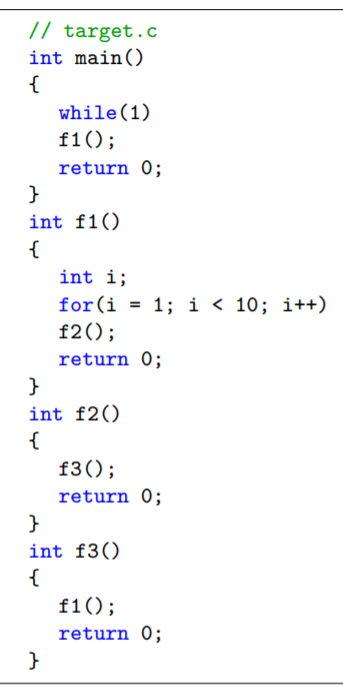
\includegraphics[height=8cm,width=10cm]{b.png}
\caption{ توربین بادی 12 کیلو‌وات (ساخته‌شده به وسیله‌ی چارلز فرانسیس براش) \cite{b1}.}
\label{wt}
\centering
\end{figure}

یک نمونه از توربین‌های بادی اولیه در شکل~\ref{wt} نشان داده شده است. در \cite{a1}، یک مدل معیار\LTRfootnote{ Benchmark Model } برای پیاده‌سازی و مقایسه‌ی روش‌های تشخیص و جداسازی عیب در توربین‌های بادی ارائه شده است. این مدل معیار، یک توربین بادی سه پره‌ی  محور افقی با سرعت متغیر و توان مجاز 4/8 مگا‌وات را که به کنترل گام\LTRfootnote{ Pitch Control }(تغییر زاویه‌ی پره‌‌های توربین بادی حول محور طولی پره‌ها با اعمال فرامین کنترلی) نیز مجهز است، شبیه‌سازی می‌کند. هدف از ارائه‌ی این مدل، بوجود آوردن یک فضای مناسب برای مقایسه و آزمایش روش‌های مختلف تشخیص و جداسازی عیوب بر روی توربین است. از این مدل می‌توان برای مقایسه‌ی روش‌های سازش با عیب که در زمینه‌ی توربین بادی ارائه شده‌اند، استفاده کرد. تعداد زیادی از تحقیقاتی که در سال‌های گذشته در زمینه‌ی تشخیص و جداسازی عیب و همچنین سازش با عیب انجام گرفته است، طرح‌های پیشنهادی خود را بر روی این مدل آزمایش و مقایسه کرده‌اند. 

یکی از اجزای توربین بادی که در معرض عیب قرار دارد، محرک گام پره‌ی توربین می‌باشد. هر یک از پره‌های توربین بادی توسط یک محرک کنترل می‌شوند و با وقوع عیب در  محرک‌ گام هر پره، موقعیت گام آن پره با خطای زیادی مواجه می‌شود. برای حل این مساله،  در \cite{a10} یک روش جبران مبتنی بر تخصیص کنترل\LTRfootnote{ Control Allocation } ارائه شده است. تخصیص کنترل، یکی از رایج‌ترین روش‌های کنترل انعطاف‌پذیر در برابر عیب است. در روش پیشنهادی، گشتاوری که بر اثر عیب یکی از محرک‌ها اتلاف می‌شود، توسط اعمال قانون کنترلی به دو محرک دیگر جبران می‌گردد و توان مطلوب توربین بادی قابل دست‌یابی است.



\section{اهداف و دستاوردهای تحقیق}
از آنجایی که کنترل‌کننده‌ی توربین بادی برای تعیین ناحیه‌ی کنترلی و اعمال دستورات کنترلی مناسب، از اطلاعات حاصل از حس‌گر‌ها استفاده می‌کند؛ وقوع عیب در حس‌گر‌ها می‌تواند سبب تغذیه‌ی اشتباه کنترل‌کننده‌ی توربین شود. در صورتی که کنترل‌کننده‌ی توربین از اطلاعات اشتباه حس‌گر‌ها استفاده کند، دستورات کنترلی که به محرک‌ها اعمال می‌کند اشتباه خواهند بود. این امر سبب می‌شود تا با گذشت زمان، کل سیستم تحت تاثیر قرار گرفته و از حالت بدون عیب فاصله بگیرند. 

در این پایان‌نامه، طرحی پیشنهاد شده است که باعث جلوگیری از کاهش راندمان سیستم، در صورت وجود عیب در حس‌گر‌های اطراف پیشرانه‌ی توربین بادی خواهد شد. در این تحقیق، تشخیص زمان و مکان وقوع عیب، شدت عیب و جداسازی عیب‌ها از یکدیگر به صورت آنلاین مورد بررسی قرار گرفته است. با فرض این که حس‌گر‌های سرعت روتور و ژنراتور و همچنین گشتاور ژنراتور (حس‌گر‌های اطراف پیشرانه‌ی توربین بادی) دچار عیب شوند، با مدل‌سازی مناسب پیشرانه، رویتگر‌هایی را برای تخمین حالت و تولید مانده طراحی کرده و با کمک این رویتگر‌ها (که از نوع رویتگر‌های ورودی ناشناخته هستند)، برای هر یک از حس‌گر‌ها به طور جداگانه سیگنال آشکارسازی عیب تولید می‌کنیم. 

آشکارسازی آنلاین  و سازش با عیوب حس‌گر که در این پایان‌نامه ارائه شده است، بر روی مدل معیار توربین بادی پیاده‌سازی شده و با روش‌های دیگر مورد مقایسه قرار گرفته است. نتایج شبیه‌سازی، بهبود عملکرد سیستم را در صورت بکار‌گیری روش پیشنهادی نشان خواهد داد. 


\section{ساختار پایان‌نامه}
در فصل دوم  به طور مختصر با تاریخچه‌ی انرژی باد آشنا خواهیم شد. همچنین نحوه‌ی عملکرد توربین بادی و اجزای تشکیل‌دهنده‌ی توربین را نیز در این فصل بررسی خواهیم کرد. در پایان این فصل با انواع تقسیم‌بندی‌های توربین‌های بادی از نظر مکان نصب و نحوه‌ی اتصال به شبکه و قرار‌گیری روتور توربین به طور مختصر آشنا خواهیم شد.

در فصل پایانی به بیان نتایج پایان‌نامه و ارائه چند پیشنهاد پرداخته خواهد شد. 


% Chapter 2
\chapter{مفاهیم پایه}

%%%%%%%%%%%%%%%%%%%%%%%%%%%%%%%
%%%%%%%%%%%%%%%%%%%%%%%%%%%%%%%
\section{سیستم‌های هم‌زمان}
همزمانی\LTRfootnote{concurrency} به معنای انجام چند عملیات در یک زمان واحد است. هنگامی که در یک سیستم، چند نخ\LTRfootnote{thread} اجرایی به صورت موازی\LTRfootnote{parallel}  اجرا شوند، همزمانی رخ می‌دهد. هنگامی که همزمانی رخ می‌دهد، ممکن است برای مثال چند نخ اجرایی به صورت همزمان  به یک منبع داده در سیستم دسترسی پیدا کنند. در این صورت، امکان بروز یک سری مشکلات احتمالی وجود دارد. به این دلیل است که به سیستم‌های هم‌زمان\LTRfootnote{concurrent systems} توجه ویژه‌ای می‌شود.

%%%%%%%%%%%%%%%%%%%%%%%%%%%%%%%
\section{سیستم‌های زمان-واقعی}
سیستم‌های زمان-واقعی\LTRfootnote{real-time systems} ، سیستم‎هایی هستند که انجام عملیات و پردازش‌ها توسط آن‌ها باید در کسری از ثانیه رخ‌دهد. این سیستم‌ها محدودیت زمانی مشخصی دارند و باید آن را تضمین کنند. به این ترتیب، یک سیستم زمان-واقعی یا یک عملیات را در آن زمان معین انجام می‌دهد، یا با شکست\LTRfootnote{failure}  مواجه می‌شود.

%%%%%%%%%%%%%%%%%%%%%%%%%%%%%%%%%%%%
\section{Spin}
Spin \cite{1} محبوب ترین ابزار در جهان برای تشخیص نقص های نرم افزاری در طراحی سیستم های همزمان است. با این حال، کد های Promela را به عنوان ورودی در یافت می‌کند و نمی‌تواند برنامه های C را مستقیماً بررسی کند. بنابراین همواره سعی می‌شود تا روش‌هایی واسطه ای برای تبدیل کد C به کد Promela ابداع شود؛ تا امکان توصیف و بررسی کدهای C برای یافتن مشکلات احتمالی در برنامه های همزمان و سیستم های موازی با استفاده از Spin میسر شود.
\\
این ابزار که به صورت متن‌باز\LTRfootnote{open source}  و رایگان دردسترس همه‌ی افراد است؛ قابلیت اجرا برروی سیستم‌عامل‌های Unix ، Linux ، Mac ، Solaris و بسیاری از نسخه‌های Windows را دارد. همچنین، علاوه بر اینکه با کمک خط فرمان\LTRfootnote{command line}  قابل استفاده‌است، دارای یک رابط کاربری گرافیکی کاربرپسند\LTRfootnote{user-friendly GUI}  است، که کار با آن را راحت‌تر می‌کند. در این پژوهش، در چندین مورد، از این ابزار قوی برای وارسی و تایید\LTRfootnote{verification}  مدل‌های Promela استفاده شده‌است. به علاوه، یک راهنمای بسیار کاربردی درباره‌ی نحوه‌ی نصب و اجرای قابلیت‌های مختلف آن دردسترس ‌است.

%%%%%%%%%%%%%%%%%%%%%%%%%%%%%%%%%%%%

\section{زبان Promela}
Promela \cite{4} یک زبان مدل‌سازی فرایند است، که از آن برای تست و وارسی منطق سیستم های موازی استفاده می‌شود. برای وارسی و تایید صحت مدل‌های نوشته شده در این زبان، از ابزار Spin استفاده می‌شود.
\\
این زبان از نظر قواعد نحوی\LTRfootnote{syntactic rules} ، به زبان C شباهت‌ دارد. به همین دلیل است که می‌توان بسیاری از ساختمان‌داده‌های\LTRfootnote{data structures}  معمول و ساده‌ی موجود در زبان C را به طور مستقیم به همان نوع ساختمان‌داده‌ها در Promela ترجمه کرد. از جمله تفاوت‌های موجود در بین این دو زبان، که در این پژوهش نیز مورد بررسی قرار گرفته‌است، عدم وجود توابع \LTRfootnote{functions}  (با همان رفتار مشابه توابع در زبان C ) در زبان Promela است. بنابراین، توابع موجود در زبان C باید به رویه‌ \LTRfootnote{proctype} ها در زبان Promela ترجمه شوند و با استفاده از امکانات دیگری که در این زبان وجود دارد، عملکرد توابع زبان C به خوبی شبیه‌سازی شود. در بخش های آتی، دقیق‌تر به این موضوع پرداخته‌خواهدشد.

%%%%%%%%%%%%%%%%%%%%%%%%%%%%%
\section{زبان \lr{ (Specification and Description Language) SDL}} 
SDL یک زبان مدل‌سازی است که برای توصیف سیستم‌های زمان-واقعی استفاده می‌شود. نمودار SDL فرایند مدل‌سازی را نشان می‌دهد. این زبان می‌تواند به طور گسترده‌ در سیستم‌های خودرو، هوانوردی، ارتباطات، پزشکی و مخابرات استفاده شود.


% Chapter 3
\chapter{سیستم های مشابه}

%%%%%%%%%%%%%%%%%%%%%%%%%%%%%%%
%%%%%%%%%%%%%%%%%%%%%%%%%%%%%%%
\section{ابزار Modex}
Modex \cite{2}  ابزاری است که حدوداَ بیست سال پیش توسط جرارد هالزمن \LTRfootnote{Gerard Holzmann} توسعه یافته‌است. این ابزار  با استفاده از زبان C نوشته شده‌است و هدف آن استخراج خودکار مدل به زبان Promela از کد C است. این ابزار برنامه‌های  معمولی C را به شیوه‌ی معقولی به زبان Promela ترجمه می‌کند. اما هنوز محدودیت های آشکاری دارد‌؛ یعنی فقط از Promela به‌صورت محدودی استفاده می‌کند. به عنوان مثال، اشاره‌گر\LTRfootnote{pointer}ها را اداره نمی کند و هیچ فراخوانی رویه\LTRfootnote{procedure call} ای ندارد. از آنجا که Promela به اندازه‌ی زبان C قدرتمند نیست، بسیاری از انواع داده های انعطاف پذیر و عملکردهای مبتکرانه ی موجود در زبان C را نمی‌توان مستقیماً به Promela  ترجمه کرد. بنابراین، Modex  این کدهای ترجمه ناپذیر را به صورت مستقیم در کد Promela تعبیه می‌کند و به این صورت به این نوع امکانات زبان C رسیدگی می‌کند. قطعات کد تعبیه‌شده\LTRfootnote{embedded} را نمی‌توان با SPIN بررسی کرد؛ نه در مرحله تجزیه\LTRfootnote{parsing phase} و نه در مرحله تأیید\LTRfootnote{verification phase}. بنابراین، به آن‌ها به صورت کورکورانه اعتماد می‌شود، و از متن مدل، در کدی که Spin ایجاد می‌کند، کپی می‌شوند. به طور خاص، اگر یک قطعه کد C تعبیه‌شده شامل یک عملیات غیرمجاز باشد؛ مانند عملیات تقسیم بر صفر یا یک اشاره‌گر به فضای خالی\LTRfootnote{NULL pointer}؛ نتیجه می‌تواند در حالی که مدل بررسی می‌شود، مخرب باشد. برای ترجمه‌ی این بخش‌های کد C به Promela ، برای اینکه بتوان آن‌ها را با Spin مورد وارسی قرارداد، باید از روش‌های خلاقانه تری نسبت به Modex استفاده کرد. یکی از مهم‌ترین محدودیت های Modex ، ترجمه‌ی اشاره‌گرهاست. Modex در این حد  اشار‌ه‌گرها را کنترل می‌کند، که هنگام استفاده از آن‌ها، تاکید\LTRfootnote{assertion}هایی را ایجاد می‌کند؛ اما فقط برای اطمینان از این هستند که اشاره‏گرها به فضای خالی از حافظه ارجاع‌ داده‌نشده‌باشند. بنابراین، سعی نمی‌کند جزئیات را بررسی کند و مشکلات احتمالی هر اشاره‌گر را پیدا‌کند، و فقط به بررسی عدم اشاره‌ به فضای خالی از حافظه کفایت می‌کند.


%%%%%%%%%%%%%%%%%%%%%%%%%%%%%%%%%%%%
\section{ابزار \lr{JPF(Java PathFinder)}}
JPF \cite{3} در ابتدا در سال 1999 به عنوان مترجمی از زیرمجموعه‌ای از Java - شامل ایجاد شی پویا\LTRfootnote{ dynamic object creation }، وراثت\LTRfootnote{ inheritance }، استثنائات\LTRfootnote{ exceptions } و عملیات مربوط به نخ های اجرا\LTRfootnote{ thread operations } - به Promela توسعه داده‌شد و از Spin برای بررسی مدل ترجمه شده استفاده‌کرد. این ابزار سعی می‌کرد کدهای Java را به کدهای با عملکردهای مشابه در Promela ترجمه کند. چند سال بعد، به عنوان یک ماشین مجازی Java \LTRfootnote{JVM} توسعه داده‌شد، که به طور خودکار تمام مسیرهای اجرای احتمالی یک برنامه را برای یافتن نقض ویژگی ها \LTRfootnote{violations of properties} مانند بن بست \LTRfootnote{deadlock} ها یا موارد استثنایی کنترل نشده \LTRfootnote{unhandled exceptions} مورد بررسی قرار‌می‌دهد.

%%%%%%%%%%%%%%%%%%%%%%%%%%%%%%%%%%%%
\section{ابزار \lr{SDL2PML}}
\lr{SDL2PML} \cite{5} ابزاری برای تولید خودکار مدل Promela از SDL است. کاملاً مستقل است و به هیچ ابزار خارجی متکی نیست. به صورت خودکار مدل هایی را تولید می‌کند که می‌توان با Spin آن‎ها را ارزیابی کرد. مدل‌هایی که تولید می‌کند، می‌توانند شامل کد C تعبیه‌شده‌باشند؛ یعنی از این مزیت برخوردار است که بخش‌هایی از کد را که نمی‌تواند ترجمه کند، به صورت کدهای تعبیه‌شده ی C در کد Promela قرار دهد. این ابزار با موفقیت در مواردی برای تولید مدل در کاربردهای دنیای واقعی مورد استفاده قرار‌گرفته‌است. کاستی قابل‌توجهی که در این ابزار وجود دارد، عدم پشتیبانی برنامه‌های با اجرای چندخطی\LTRfootnote{multi-threaded execution}  است. 


%%%%%%%%%%%%%%%%%%%%%%%%%%%%%%%%%%%%
\section{\lr{ke thesis}}
\lr{Ke Jiang} مقاله‌ای تحت عنوان \lr{Model Checking C Programs by Translating C to Promela} \cite{6} ارائه کرده‌است؛ که در آن روش‌هایی موثر برای استخراج کد Promela از کد C معرفی شده‌‌است. این روش‌ها با تمرکز بر روی ضعف‌های سایر ابزارهایی که از پیش وجود داشتند و برای رفع آن کاستی‌ها ارائه شده‌اند. 


%%%%%%%%%%%%%%%%%%%%%%%%%%%%%%%%%%%%
\section{نتیجه‌گیری}
با توجه به بررسی‌های صورت‌گرفته بر روی سیستم‌های مشابه، ابزار Modex بهترین ابزار دردسترس برای تبدیل کد C به Promela تشخیص‌داده‌شد. بنابراین، تصمیم بر بهبود برخی عملکردهای آن گرفته‌شد. می‌توان برای این کار، از روش‌های موجود در مقاله‌ی معرفی شده در بخش 3.4 الهام گرفت.

% Chapter 4
\chapter{روش پیشنهادی}

%%%%%%%%%%%%%%%%%%%%%%%%%%%%%%%
%%%%%%%%%%%%%%%%%%%%%%%%%%%%%%%
\section{شرح مسئله}
همانطورکه پیش‌تر بیان‌شد، یکی از نقاط ضعف Modex مربوط به عدم فراخوانی هیچ گونه رویه ای است. این موجب می‌شود تا تبدیل توابع کد C به رویه ها در کد Promela ، در برخی کدهای پیچیده‌تر با مشکل جدی مواجه شود. برای مثال، در برنامه‌های با فراخوانی‌های پیچیده‌تر توابع در زبان C ، ترتیب اجرای رویه های کد Promela تولید شده، مطابق با ترتیب اجرای صحیح توابع کد C اولیه نخواهدبود. برای درک بهتر مسئله، در ادامه با بیان یک مثال، این مشکل شرح داده‌خواهدشد و راه حلی با تمرکز بر روی همین مثال ارائه خواهدشد.
شکل 4-1 که کد به زبان C را نشان می‌دهد، در نظر بگیرید.

 \begin{figure}
	\centering
	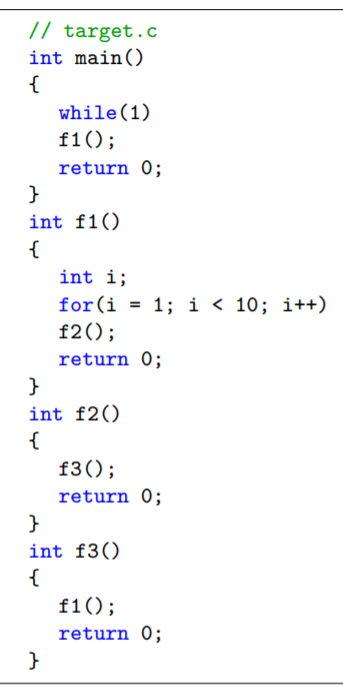
\includegraphics[height=10cm,width=6cm]{b.png}
	\caption{کد به زبان C}
	\centering
\end{figure}


%\hspace{0.5cm}
%\begin{latin}
%\begin{lstlisting}
%	// target.c
%	int main()
%	{
%		while(1)
%		f1();
%		return 0;
%	}
%	int f1()
%	{
%		int i;
%		for(i = 1; i < 10; i++)
%		f2();
%		return 0;
%	}
%	int f2()
%	{
%		f3();
%		return 0;
%	}
%	int f3()
%	{
%		f1();
%		return 0;
%	}
%\end{lstlisting}
%\end{latin}


\section{مدل سازی با Modex}
می خواهیم این کد را به Promela  ترجمه کنیم،
\subsection{حالت اول}
اگر فایل \lr{target.prx} نداشته باشیم(یا این فایل خالی باشد)، و یا اینکه محتوای آن مانند کد نشان داده شده در شکل 4-2 باشد، کد Promela تولید شده توسط Modex ، به صورت کد نشان داده شده در دو شکل 4-3 و 4-4 خواهدبود.

 \begin{figure}
	\centering
	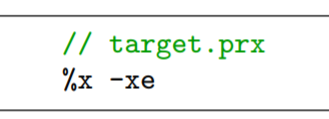
\includegraphics[height=1.5cm,width=4cm]{c.png}
	\caption{محتوای فایل .prx}
	\centering
\end{figure}

% \hspace{0.5cm}
% \begin{latin}
% 	\begin{lstlisting}
% 		// target.prx
% 		%x -xe
% 	\end{lstlisting}
% \end{latin}


 \begin{figure}
	\centering
	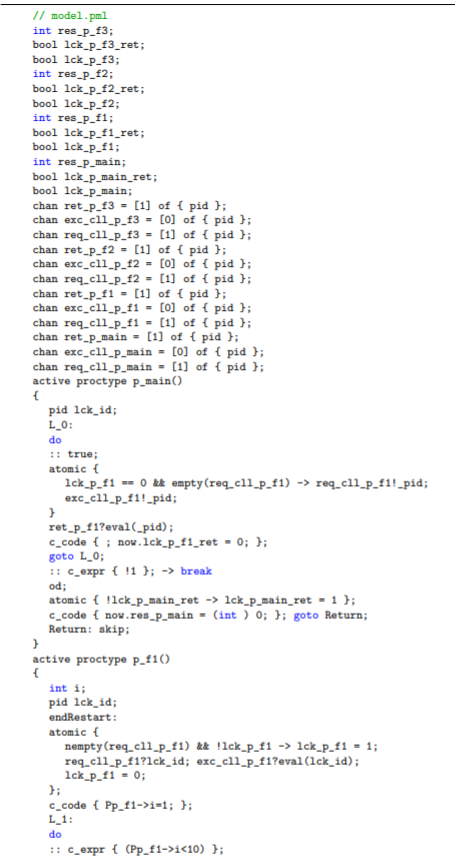
\includegraphics[height=25cm,width=12cm]{d1.png}
	\caption{فایل نتیجه Modex}
	\centering
\end{figure}

 \begin{figure}
	\centering
	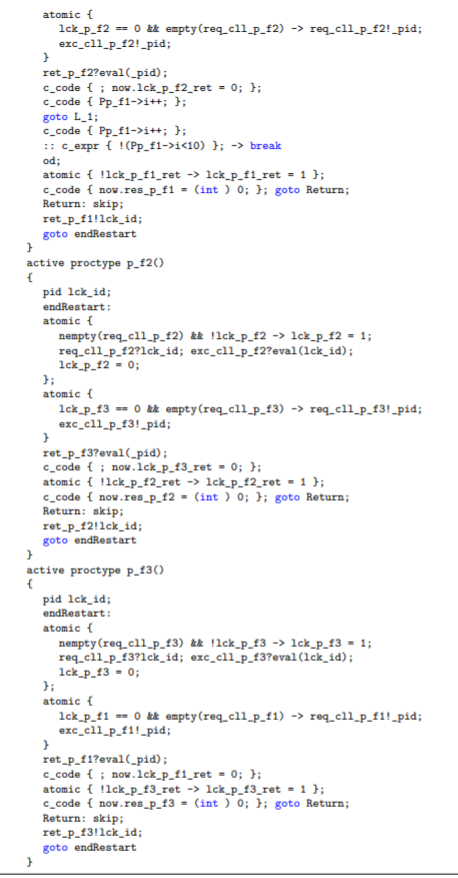
\includegraphics[height=25cm,width=12cm]{d2.png}
	\caption{ادامه فایل نتیجه Modex}
	\centering
\end{figure}

%\hspace{0.5cm}
%\begin{latin}
%	\begin{lstlisting}
%		// model.pml
%		int res_p_f3;
%		bool lck_p_f3_ret;
%		bool lck_p_f3;
%		int res_p_f2;
%		bool lck_p_f2_ret;
%		bool lck_p_f2;
%		int res_p_f1;
%		bool lck_p_f1_ret;
%		bool lck_p_f1;
%		int res_p_main;
%		bool lck_p_main_ret;
%		bool lck_p_main;
%		chan ret_p_f3 = [1] of { pid };
%		chan exc_cll_p_f3 = [0] of { pid };
%		chan req_cll_p_f3 = [1] of { pid };
%		chan ret_p_f2 = [1] of { pid };
%		chan exc_cll_p_f2 = [0] of { pid };
%		chan req_cll_p_f2 = [1] of { pid };
%		chan ret_p_f1 = [1] of { pid };
%		chan exc_cll_p_f1 = [0] of { pid };
%		chan req_cll_p_f1 = [1] of { pid };
%		chan ret_p_main = [1] of { pid };
%		chan exc_cll_p_main = [0] of { pid };
%		chan req_cll_p_main = [1] of { pid };
%		active proctype p_main()
%		{
%			pid lck_id;
%			L_0:
%			do
%			:: true;
%			atomic {
%				lck_p_f1 == 0 && empty(req_cll_p_f1) -> req_cll_p_f1!_pid;
%				exc_cll_p_f1!_pid;
%			}
%			ret_p_f1?eval(_pid);
%			c_code { ; now.lck_p_f1_ret = 0; };
%			goto L_0;
%			:: c_expr { !1 }; -> break
%			od;
%			atomic { !lck_p_main_ret -> lck_p_main_ret = 1 };
%			c_code { now.res_p_main = (int ) 0; }; goto Return;
%			Return: skip;
%		}
%		active proctype p_f1()
%		{
%			int i;
%			pid lck_id;
%			endRestart:
%			atomic {
%				nempty(req_cll_p_f1) && !lck_p_f1 -> lck_p_f1 = 1;
%				req_cll_p_f1?lck_id; exc_cll_p_f1?eval(lck_id);
%				lck_p_f1 = 0;
%			};
%			c_code { Pp_f1->i=1; };
%			L_1:
%			do
%			:: c_expr { (Pp_f1->i<10) };
%			atomic {
%				lck_p_f2 == 0 && empty(req_cll_p_f2) -> req_cll_p_f2!_pid;
%				exc_cll_p_f2!_pid;
%			}
%			ret_p_f2?eval(_pid);
%			c_code { ; now.lck_p_f2_ret = 0; };
%			c_code { Pp_f1->i++; };
%			goto L_1;
%			c_code { Pp_f1->i++; };
%			:: c_expr { !(Pp_f1->i<10) }; -> break
%			od;
%			atomic { !lck_p_f1_ret -> lck_p_f1_ret = 1 };
%			c_code { now.res_p_f1 = (int ) 0; }; goto Return;
%			Return: skip;
%			ret_p_f1!lck_id;
%			goto endRestart
%		}
%		active proctype p_f2()
%		{
%			pid lck_id;
%			endRestart:
%			atomic {
%				nempty(req_cll_p_f2) && !lck_p_f2 -> lck_p_f2 = 1;
%				req_cll_p_f2?lck_id; exc_cll_p_f2?eval(lck_id);
%				lck_p_f2 = 0;
%			};
%			atomic {
%				lck_p_f3 == 0 && empty(req_cll_p_f3) -> req_cll_p_f3!_pid;
%				exc_cll_p_f3!_pid;
%			}
%			ret_p_f3?eval(_pid);
%			c_code { ; now.lck_p_f3_ret = 0; };
%			atomic { !lck_p_f2_ret -> lck_p_f2_ret = 1 };
%			c_code { now.res_p_f2 = (int ) 0; }; goto Return;
%			Return: skip;
%			ret_p_f2!lck_id;
%			goto endRestart
%		}
%		active proctype p_f3()
%		{
%			pid lck_id;
%			endRestart:
%			atomic {
%				nempty(req_cll_p_f3) && !lck_p_f3 -> lck_p_f3 = 1;
%				req_cll_p_f3?lck_id; exc_cll_p_f3?eval(lck_id);
%				lck_p_f3 = 0;
%			};
%			atomic {
%				lck_p_f1 == 0 && empty(req_cll_p_f1) -> req_cll_p_f1!_pid;
%				exc_cll_p_f1!_pid;
%			}
%			ret_p_f1?eval(_pid);
%			c_code { ; now.lck_p_f1_ret = 0; };
%			atomic { !lck_p_f3_ret -> lck_p_f3_ret = 1 };
%			c_code { now.res_p_f3 = (int ) 0; }; goto Return;
%			Return: skip;
%			ret_p_f3!lck_id;
%			goto endRestart
%		}
%	\end{lstlisting}
%\end{latin}

حال برای بررسی این مدل و مسیرهای اجرایی ممکن در آن، از Spin استفاده می‌کنیم.
\\
به طور کلی 5 مسیر اجرایی ممکن به شرح زیر برای مدل تولید شده، محتمل است:

\begin{enumerate}
	\item به ترتیب از راست به چپ main ، f1  ، f2  و درنهایت f3 اجرا می‌‌شود. و برنامه به اتمام می‌رسد.
	\item به ترتیب از راست به چپ main ، f1  ،  main ، f1  ، f2  و درنهایت f3 اجرا می‌‌شود. و برنامه به اتمام می‌رسد.
	\item به ترتیب از راست به چپ main ، f1  ،  main ، و درنهایت f1 اجرا می‌‌شود. و برنامه به اتمام می‌رسد.
	\item به ترتیب از راست به چپ main ، f1  ، و درنهایت main اجرا می‌‌شود. و برنامه به اتمام می‌رسد.
	\item فقط main اجرا می‌‌شود. و برنامه به اتمام می‌رسد.
\end{enumerate}
برای مثال، مسیر اجرایی چهارم به صورت شکل 4-5 است:

 \begin{figure}
	\centering
	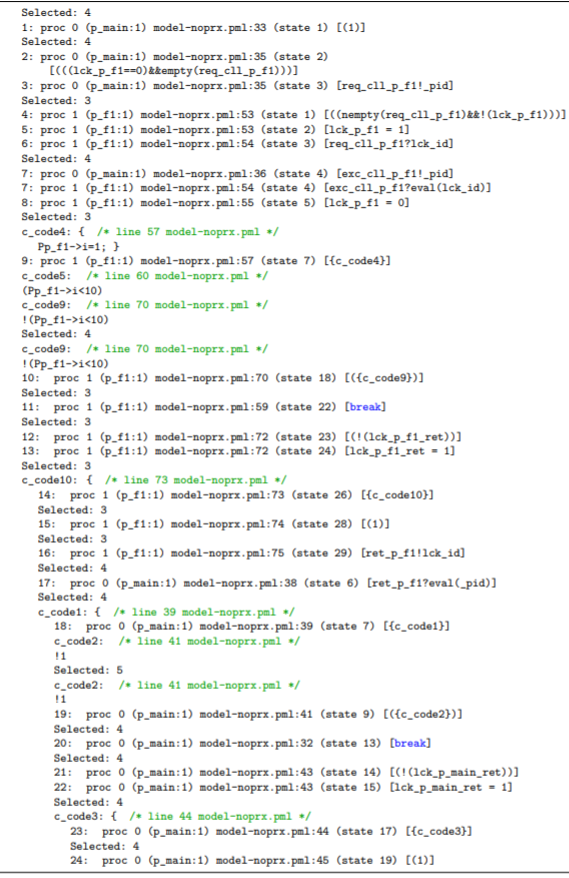
\includegraphics[height=25cm,width=16cm]{e.png}
	\caption{مسیر اجرایی}
	\centering
\end{figure}

%\begin{latin}
%	\begin{lstlisting}
%	Selected: 4
%	1:	proc  0 (p_main:1) model-noprx.pml:33 (state 1)	[(1)]
%	Selected: 4
%	2:	proc  0 (p_main:1) model-noprx.pml:35 (state 2)	[(((lck_p_f1==0)&&empty(req_cll_p_f1)))]
%	3:	proc  0 (p_main:1) model-noprx.pml:35 (state 3)	[req_cll_p_f1!_pid]
%	Selected: 3
%	4:	proc  1 (p_f1:1) model-noprx.pml:53 (state 1)	[((nempty(req_cll_p_f1)&&!(lck_p_f1)))]
%	5:	proc  1 (p_f1:1) model-noprx.pml:53 (state 2)	[lck_p_f1 = 1]
%	6:	proc  1 (p_f1:1) model-noprx.pml:54 (state 3)	[req_cll_p_f1?lck_id]
%	Selected: 4
%	7:	proc  0 (p_main:1) model-noprx.pml:36 (state 4)	[exc_cll_p_f1!_pid]
%	7:	proc  1 (p_f1:1) model-noprx.pml:54 (state 4)	[exc_cll_p_f1?eval(lck_id)]
%	8:	proc  1 (p_f1:1) model-noprx.pml:55 (state 5)	[lck_p_f1 = 0]
%	Selected: 3
%	c_code4:	{ 	/* line 57 model-noprx.pml */
%		Pp_f1->i=1;  }
%	9:	proc  1 (p_f1:1) model-noprx.pml:57 (state 7)	[{c_code4}]
%	c_code5:		/* line 60 model-noprx.pml */
%	(Pp_f1->i<10) 
%	c_code9:		/* line 70 model-noprx.pml */
%	!(Pp_f1->i<10) 
%	Selected: 4
%	c_code9:		/* line 70 model-noprx.pml */
%	!(Pp_f1->i<10) 
%	10:	proc  1 (p_f1:1) model-noprx.pml:70 (state 18)	[({c_code9})]
%	Selected: 3
%	11:	proc  1 (p_f1:1) model-noprx.pml:59 (state 22)	[break]
%	Selected: 3
%	12:	proc  1 (p_f1:1) model-noprx.pml:72 (state 23)	[(!(lck_p_f1_ret))]
%	13:	proc  1 (p_f1:1) model-noprx.pml:72 (state 24)	[lck_p_f1_ret = 1]
%	Selected: 3
%	c_code10:	{ 	/* line 73 model-noprx.pml */
%	14:	proc  1 (p_f1:1) model-noprx.pml:73 (state 26)	[{c_code10}]
%	Selected: 3
%	15:	proc  1 (p_f1:1) model-noprx.pml:74 (state 28)	[(1)]
%	Selected: 3
%	16:	proc  1 (p_f1:1) model-noprx.pml:75 (state 29)	[ret_p_f1!lck_id]
%	Selected: 4
%	17:	proc  0 (p_main:1) model-noprx.pml:38 (state 6)	[ret_p_f1?eval(_pid)]
%	Selected: 4
%	c_code1:	{ 	/* line 39 model-noprx.pml */
%	18:	proc  0 (p_main:1) model-noprx.pml:39 (state 7)	[{c_code1}]
%	c_code2:		/* line 41 model-noprx.pml */
%	!1 
%	Selected: 5
%	c_code2:		/* line 41 model-noprx.pml */
%	!1 
%	19:	proc  0 (p_main:1) model-noprx.pml:41 (state 9)	[({c_code2})]
%	Selected: 4
%	20:	proc  0 (p_main:1) model-noprx.pml:32 (state 13)	[break]
%	Selected: 4
%	21:	proc  0 (p_main:1) model-noprx.pml:43 (state 14)	[(!(lck_p_main_ret))]
%	22:	proc  0 (p_main:1) model-noprx.pml:43 (state 15)	[lck_p_main_ret = 1]
%	Selected: 4
%	c_code3:	{ 	/* line 44 model-noprx.pml */
%	23:	proc  0 (p_main:1) model-noprx.pml:44 (state 17)	[{c_code3}]
%	Selected: 4
%	24:	proc  0 (p_main:1) model-noprx.pml:45 (state 19)	[(1)]
%	\end{lstlisting}
%\end{latin}

اگر به برنامه C موردنظر توجه کنید، متوجه می‌شوید که این برنامه در تابع اصلی (main) دارای یک حلقه‌ی بی‌نهایت است و منطقاً نباید هیچ‌گاه فراخوانی توابع به پایان برسد. ولی در مدل Promela تولید شده، در همه‌ی حالت‌ها فراخوانی توابع تمام می‌شود و مدل‌سازی به پایان می‌رسد.
\\
حالا اگر به مدل Promela تولید شده توجه کنید، متوجه می‌شوید که این اتمام زودهنگام فراخوانی‌ها به همان دلیل عدم امکان فراخوانی رویه‌ها در کد تولیدی Modex ، که پیش‌تر عنوان شد، است. تمام رویه‌های تولید شده در این کد، به صورت فعال\LTRfootnote{active proctype}  استفاده شده‌اند و با استفاده از کانال‌های هم‌گام‌ساز \LTRfootnote{synchronization channels}   سعی شده که تا حدی ابتدایی ترتیب اجرای آن‌ها رعایت شود. ولی با توجه به اینکه رویه‌های از ابتدا فعال، فقط به صورت یک نمونه\LTRfootnote{instance}   از آن رویه عمل می‌کنند، این ساختار تولید مدل نمی‌تواند در یک شرایط پیچیده از فراخوانی رویه ها، پاسخگوی اجرای درست رویه‌ها باشد.


\subsection{حالت دوم}
اگر محتوای فایل \lr{target.prx} آن مانند کد نشان داده شده در شکل 4-6 باشد، کد Promela تولید شده توسط Modex ، به صورت کد نشان داده شده در شکل 4-7 خواهدبود.

 \begin{figure}
	\centering
	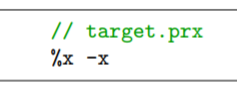
\includegraphics[height=1.5cm,width=4cm]{f.png}
	\caption{محتوای فایل .prx}
	\centering
\end{figure}


%\hspace{0.5cm}
%\begin{latin}
%	\begin{lstlisting}
%		// target.prx
%		%x -x
%	\end{lstlisting}
%\end{latin}

 \begin{figure}
	\centering
	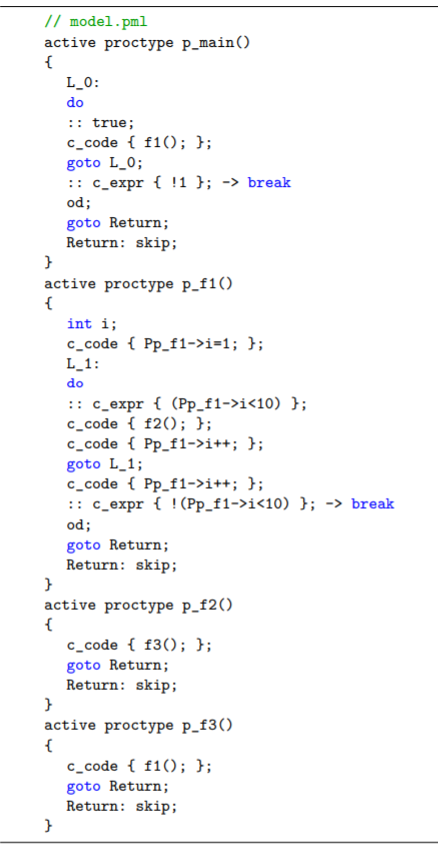
\includegraphics[height=25cm,width=12cm]{g.png}
	\caption{فایل نتیجه Modex}
	\centering
\end{figure}

%\hspace{0.5cm}
%\begin{latin}
%	\begin{lstlisting}
%		// model.pml
%		active proctype p_main()
%		{
%			L_0:
%			do
%			:: true;
%			c_code { f1(); };
%			goto L_0;
%			:: c_expr { !1 }; -> break
%			od;
%			goto Return;
%			Return: skip;
%		}
%		active proctype p_f1()
%		{
%			int i;
%			c_code { Pp_f1->i=1; };
%			L_1:
%			do
%			:: c_expr { (Pp_f1->i<10) };
%			c_code { f2(); };
%			c_code { Pp_f1->i++; };
%			goto L_1;
%			c_code { Pp_f1->i++; };
%			:: c_expr { !(Pp_f1->i<10) }; -> break
%			od;
%			goto Return;
%			Return: skip;
%		}
%		active proctype p_f2()
%		{
%			c_code { f3(); };
%			goto Return;
%			Return: skip;
%		}
%		active proctype p_f3()
%		{
%			c_code { f1(); };
%			goto Return;
%			Return: skip;
%		}
%	\end{lstlisting}
%\end{latin}

در این حالت با توجه به اینکه رویه‌ها از ابتدا فعال هستند، ولی این‌بار با استفاده از کانال‌های هم‌گام‌ساز سعی در کنترل ترتیب اجرای آن‌ها نشده؛ تعداد مسیرهای اجرایی نسبت به حالت قبل هم بیشتر است و همچنان شامل مسیر درست نیست. بنابراین، این حالت نسبت به حالت اول هم عدم قطعیت\LTRfootnote{non-determinism}   بیشتری دارد.


\section{اصلاح مدل خروجی Modex}
هدف این پژوهش اصلاح همین نقص Modex که در بخش 4.2 توصیف شده؛ یعنی عدم توانایی در مدل‌سازی صحیح مدل‌های پیچیده از لحاظ توالی فراخوانی توابع است.
\\
در ادامه سعی می‌شود با ایجاد تغییراتی در کد مدل تولیدی Modex در بخش 4.2.2 ، ترتیب فراخوانی رویه‌های مدل  Promela را منطبق بر توالی اجرای تابع‌ها در کد C کرد.

\subsection{گام اول}
کد حاصل از این گام، به صورت کد نشان داده شده در شکل 4-8 است.

 \begin{figure}
	\centering
	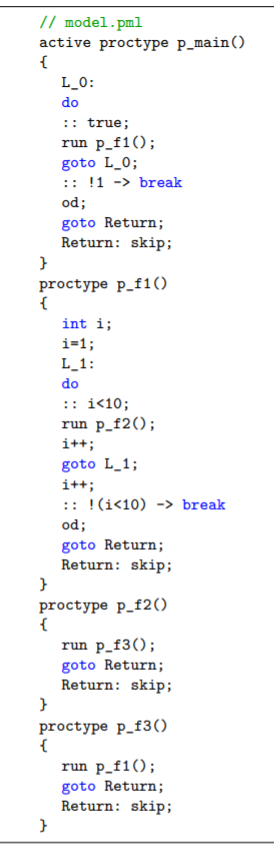
\includegraphics[height=23cm,width=7cm]{h.png}
	\caption{کد حاصل از گام اول}
	\centering
\end{figure}

%\hspace{0.5cm}
%\begin{latin}
%	\begin{lstlisting}
%		// model.pml
%		active proctype p_main()
%		{
%			L_0:
%			do
%			:: true;
%			run p_f1();
%			goto L_0;
%			:: !1 -> break
%			od;
%			goto Return;
%			Return: skip;
%		}
%		proctype p_f1()
%		{
%			int i;
%			i=1;
%			L_1:
%			do
%			:: i<10;
%			run p_f2();
%			i++;
%			goto L_1;
%			i++;
%			:: !(i<10) -> break
%			od;
%			goto Return;
%			Return: skip;
%		}
%		proctype p_f2()
%		{
%			run p_f3();
%			goto Return;
%			Return: skip;
%		}
%		proctype p_f3()
%		{
%			run p_f1();
%			goto Return;
%			Return: skip;
%		}
%	\end{lstlisting}
%\end{latin}

تغییرات ایجاد شده، شامل موارد زیر است:
\begin{enumerate}
	\item قطعه کدهای ساده‌ی مشترک بین دو زبان که در بلاک‌های تعبیه شده‌ی کد C \LTRfootnote{C-expression}    قرار داشت، از این بلاک‌ها خارج شده و به صورت کد Promela در مدل قرار گرفت. به این ترتیب، قابلیت وارسی این بخش از مدل هم توسط Spin فراهم شد.
	\item فقط تابع اصلی برنامه به صورت فعال تعریف شده‌است. بقیه‌ی توابع، در هنگام فراخوانی، با کلیداژه‌ی run اجرا می‌شوند. (برای اصلاح مشکل فراخوانی توابع، نمی‌توان از توابع inline بهره گرفت؛ چرا که در این توابع، ترتیب تعریف بدنه‌ی توابع برای امکان فراخوانی آن‌ها توسط یک‌دیگراهمیت دارد، و این موجب ایجاد محدودیت در تنوع فراخوانی های توابع می‌شود.)
\end{enumerate}

حال برای بررسی این مدل و مسیرهای اجرایی ممکن در آن، از Spin استفاده می‌کنیم.
\\
در این حالت، مشاهده می‌شود که همچنان تعداد مسیرهای اجرایی ممکن، بیش از یک مسیر است. با این حال، بهبودی که در این حالت دیده می‌شود، این است که ترتیب اجرای رویه‌ها در یکی از مسیرهای اجرایی، منطبق بر ترتیب اجرای توابع در کد C متناظر است. یعنی مدل Promela تهیه شده، علاوه بر رفتار مدل اصلی C ، رفتارهای دیگری هم از خود نشان‌ می‌دهد. در این حالت اگر به این کد  Promla به عنوان نماینده‌ی کد C مورد نظر و برای بررسی آن با استفاده از Spin تکیه کنیم، نتیجه می‌گیریم که مدل ما همواره رفتار موردنظر ما را ندارد. این نتیجه‌گیری نادرست، به دلیل وجود همان مسیرهای غیر از مسیر اصلی و درست کد C است. در این حالت اصطلاحاً گفته می‌شود که این نتیجه، منفی کاذب \LTRfootnote{false negative}    است.
\\
این مشکل به دلیل این است که وقتی یک رویه، رویه‌ی دیگری را فراخوانی می‌کند، هم خود رویه‌ی اول و هم رویه‌ی فراخوانی شده، امکان اجرا دارند. در این حالت، اطمینانی وجود ندارد که بدنه‌ی کدام‌یک از این دو تابع اجرا خواهدشد. و این قضیه موجب ایجاد عدم قطعیت در رفتار مدل می‌شود. پس باید مسیر اجرای یکی از این دو رویه بلاک شود، تا مسیر مورد انتظار اجرا شود.
\\
مسیر موردانتظار که در مسیرهای اجرایی این مدل وجود دارد، به صورت شکل 4-9 است.

 \begin{figure}
	\centering
	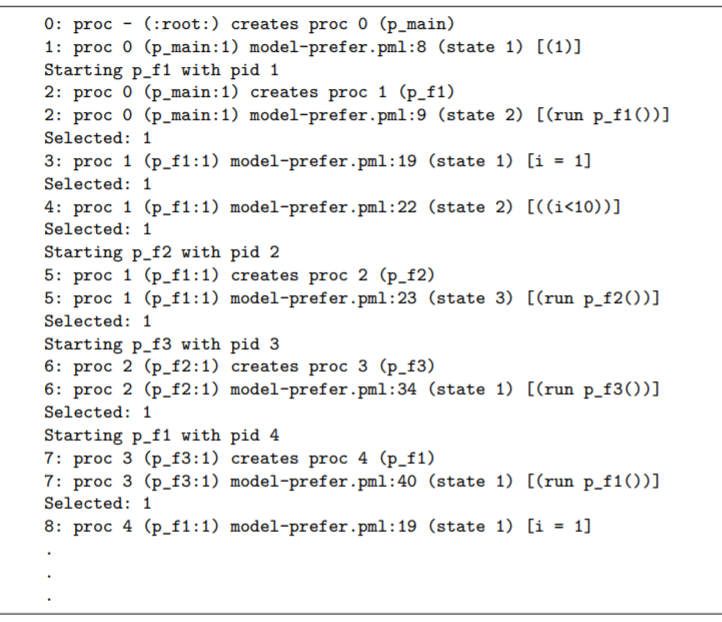
\includegraphics[height=10cm,width=15cm]{i.png}
	\caption{مسیر اجرایی مربوط به کد حاصل از گام اول}
	\centering
\end{figure}

%\hspace{0.5cm}
%\begin{latin}
%	\begin{lstlisting}
%		0:	proc  - (:root:) creates proc  0 (p_main)
%		1:	proc  0 (p_main:1) model-prefer.pml:8 (state 1)	[(1)]
%		Starting p_f1 with pid 1
%		2:	proc  0 (p_main:1) creates proc  1 (p_f1)
%		2:	proc  0 (p_main:1) model-prefer.pml:9 (state 2)	[(run p_f1())]
%		Selected: 1
%		3:	proc  1 (p_f1:1) model-prefer.pml:19 (state 1)	[i = 1]
%		Selected: 1
%		4:	proc  1 (p_f1:1) model-prefer.pml:22 (state 2)	[((i<10))]
%		Selected: 1
%		Starting p_f2 with pid 2
%		5:	proc  1 (p_f1:1) creates proc  2 (p_f2)
%		5:	proc  1 (p_f1:1) model-prefer.pml:23 (state 3)	[(run p_f2())]
%		Selected: 1
%		Starting p_f3 with pid 3
%		6:	proc  2 (p_f2:1) creates proc  3 (p_f3)
%		6:	proc  2 (p_f2:1) model-prefer.pml:34 (state 1)	[(run p_f3())]
%		Selected: 1
%		Starting p_f1 with pid 4
%		7:	proc  3 (p_f3:1) creates proc  4 (p_f1)
%		7:	proc  3 (p_f3:1) model-prefer.pml:40 (state 1)	[(run p_f1())]
%		Selected: 1
%		8:	proc  4 (p_f1:1) model-prefer.pml:19 (state 1)	[i = 1]
%		.
%		.
%		.
%	\end{lstlisting}
%\end{latin}

\subsection{گام دوم}
کد حاصل از این گام، به صورت کد نشان داده شده در دو شکل 4-10 و 4-11 است.

\begin{figure}
	\centering
	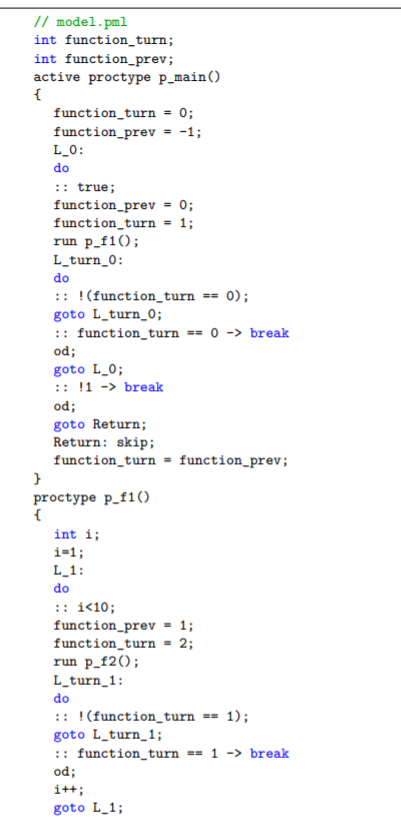
\includegraphics[height=23cm,width=10cm]{j1.png}
	\caption{کد حاصل از گام دوم}
	\centering
\end{figure}

\begin{figure}
	\centering
	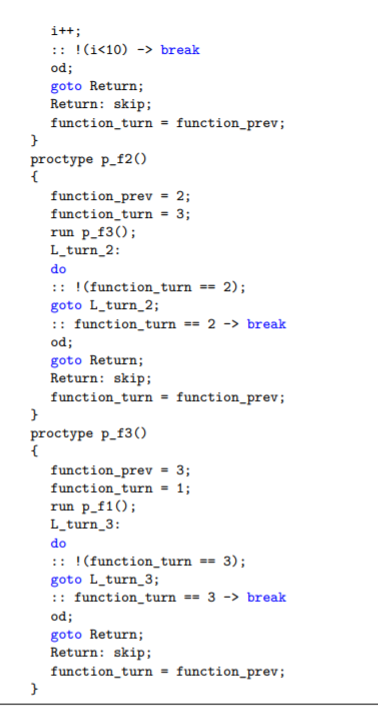
\includegraphics[height=23cm,width=11cm]{j2.png}
	\caption{ادامه کد حاصل از گام دوم}
	\centering
\end{figure}


%\hspace{0.5cm}
%\begin{latin}
%	\begin{lstlisting}
%		// model.pml
%		int function_turn;
%		int function_prev;
%		active proctype p_main()
%		{
%			function_turn = 0;
%			function_prev = -1;
%			L_0:
%			do
%			:: true;
%			function_prev = 0;
%			function_turn = 1;
%			run p_f1();
%			L_turn_0:
%			do
%			:: !(function_turn == 0);
%			goto L_turn_0;
%			:: function_turn == 0 -> break
%			od; 
%			goto L_0;
%			:: !1 -> break
%			od;
%			goto Return;
%			Return: skip;
%			function_turn = function_prev;
%		}
%		proctype p_f1()
%		{
%			int i;
%			i=1;
%			L_1:
%			do
%			:: i<10;
%			function_prev = 1;
%			function_turn = 2;
%			run p_f2();
%			L_turn_1:
%			do
%			:: !(function_turn == 1);
%			goto L_turn_1;
%			:: function_turn == 1 -> break
%			od; 
%			i++;
%			goto L_1;
%			i++;
%			:: !(i<10) -> break
%			od;
%			goto Return;
%			Return: skip;
%			function_turn = function_prev;
%		}
%		proctype p_f2()
%		{
%			function_prev = 2;
%			function_turn = 3;
%			run p_f3();
%			L_turn_2:
%			do
%			:: !(function_turn == 2);
%			goto L_turn_2;
%			:: function_turn == 2 -> break
%			od; 
%			goto Return;
%			Return: skip;
%			function_turn = function_prev;
%		}
%		proctype p_f3()
%		{
%			function_prev = 3;
%			function_turn = 1;
%			run p_f1();
%			L_turn_3:
%			do
%			:: !(function_turn == 3);
%			goto L_turn_3;
%			:: function_turn == 3 -> break
%			od; 
%			goto Return;
%			Return: skip;
%			function_turn = function_prev;
%		}
%	\end{lstlisting}
%\end{latin}

دراین گام سعی شد تا با تعریف دو متغیر عمومی\LTRfootnote{global variables}، در هنگامی که بدنه‌ی چند رویه به صورت هم‌زمان امکان اجرا داشتند، رویه‌هایی که موجب مسیر غیرمنتظره می‌‍شوند بلاک شود. یکی از متغیرها به منظور نشان دادن این است که رویه‌ای که باید اجرا شود، کدام است\LTRfootnote{function turn}. متغیر دیگر این را نشان می‌دهد که اگر رویه‌ای که در حال حاضر در آن قرار داریم به اتمام رسید، کدام رویه باید اجرا شود(با توجه به اینکه رویه‌ی حال حاضر توسط چه رویه‌ای فراخوانی شده است، تنظیم می‌شود) \LTRfootnote{function prev}.
\\
در این حالت، همچنان دو مشکل وجود دارد:
\begin{enumerate}
	\item دراین حالت، با استفاده از یک حلقه‌ سعی شده در هر رویه چک شود که آیا می‌تواند به اجرای بدنه‌ی خود ادامه دهد، یا بلاک شود. برای مثال وقتی که یک رویه، رویه‌ی دیگری را فراخوانی می‌کند، پس از آن باید وارد حلقه شود و به طور مرتب چک کند که آیا می‌تواند به اجرای بدنه‌ی خود ادامه بدهد یا خیر. اینجا مشکلی که پیش می‌آید، این است که ممکن است تمام cpu به رویه‌ی اول اختصاص پیدا کند و رویه‌ی دوم نتواند هیچ‌وقت اجرا شود. بنابراین، همچنان قطعیتی روی مسیر اجرای برنامه وجود ندارد، و مشخص نیست بدنه‌ی کدام رویه پس از آن اجرا می‌شود.
	\item مشکل دیگر، مربوط به کنترل مسیر اجرا با استفاده از متغیرهای عمومی به کارگرفته شده‌است. در این حالت، هر رویه اگر بیش از یک بار به روش های مختلف قصد اجرا داشته باشد، این متغیرها کارایی خود را از دست می‌دهند و به درستی ترتیب اجرای رویه‎‌ها را نمی‌توانند کنترل کنند. برای مثال اگر در تابع 1، تابع 2 فراحوانی شد، بدنه‌ی تابع 1 روی خط بعد از فراخوانی تابع 2 باید بلاک شود. حالا اگر دوباره از طریق تابع 2، تابع 1 فراخوانی شود، تابع 1 هم از ابتدا می‌تواند اجرا شود و هم از خطی که در میانه‌ ی بدنه‌اش بلاک شده بود؛ درحالی که ما انتظار داشتیم تابع 1 فقط از ابتدا اجرا شود و نمونه ی اولیه‌ی آن همچنان در بدنه‌ی خود بلاک بماند تا آن نمونه از تابع 1 که اجرا کرده‌بود، به اتمام برسد.
\end{enumerate}

\subsection{گام سوم}
کد حاصل از این گام، به صورت کد نشان داده شده در شکل 4-12 است.

\begin{figure}
	\centering
	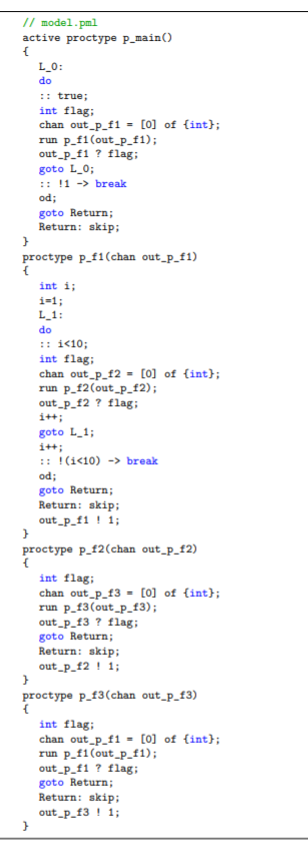
\includegraphics[height=23cm,width=9cm]{k.png}
	\caption{کد حاصل از گام سوم}
	\centering
\end{figure}


%\hspace{0.5cm}
%\begin{latin}
%	\begin{lstlisting}
%		// model.pml
%		active proctype p_main()
%		{
%			L_0:
%			do
%			:: true;
%			int flag;
%			chan out_p_f1 = [0] of {int};
%			run p_f1(out_p_f1);
%			out_p_f1 ? flag;
%			goto L_0;
%			:: !1 -> break
%			od;
%			goto Return;
%			Return: skip;
%		}
%		proctype p_f1(chan out_p_f1)
%		{
%			int i;
%			i=1;
%			L_1:
%			do
%			:: i<10;
%			int flag;
%			chan out_p_f2 = [0] of {int};
%			run p_f2(out_p_f2);
%			out_p_f2 ? flag;
%			i++;
%			goto L_1;
%			i++;
%			:: !(i<10) -> break
%			od;
%			goto Return;
%			Return: skip;
%			out_p_f1 ! 1;
%		}
%		proctype p_f2(chan out_p_f2)
%		{
%			int flag;
%			chan out_p_f3 = [0] of {int};
%			run p_f3(out_p_f3);
%			out_p_f3 ? flag;
%			goto Return;
%			Return: skip;
%			out_p_f2 ! 1;
%		}
%		proctype p_f3(chan out_p_f3)
%		{
%			int flag;
%			chan out_p_f1 = [0] of {int};
%			run p_f1(out_p_f1);
%			out_p_f1 ? flag;
%			goto Return;
%			Return: skip;
%			out_p_f3 ! 1;
%		}
%	\end{lstlisting}
%\end{latin}
در این حالت، برای کنترل ترتیب اجرای رویه‌ها، به جای استفاده از متغیرهای عمومی، از کانال‌های هم‌گام‌ساز محلی\LTRfootnote{local synchronization channels} استفاده می‌شود. به این ترتیب، هر دو مشکلی که در گام قبل با آن‌ها مواجه بودیم، برطرف می‌شود. روش استفاده از این کانال‌ها به این صورت است که در هر فراخوانی رویه، یک کانال هم‌گام‌ساز بین دو رویه فراخوانی‌کننده و فراخوانی‌شونده تنظیم می‌شود، تا اجرای این دو رویه را کنترل کند. به این ترتیب، با توجه به اینکه در هر فراخوانی رویه، یک کانال جداگانه بین نمونه‌های رویه‌ها تنظیم می‌شود، مشکل دوم گام قبل حل می‌شود. همچنین، در بدنه‌ی رویه فراخوانی‌کننده، در خط پس از خط فراخوانی، منتظر دریافت مقدار از طریق کانال می‌ماند و در همان خط بلاک می‌شود و نیاز به اختصاص مرتب cpu  نخواهدداشت و عدم قطعیتی در مسیر اجرا ایجاد نمی‌کند.
\\
تنها مسیر اجرای حاصل از مدل در این گام، که همان مسیر درست است، در شکل 4-13 نشان ‌داده‌شده‌‍است.

\begin{figure}
	\centering
	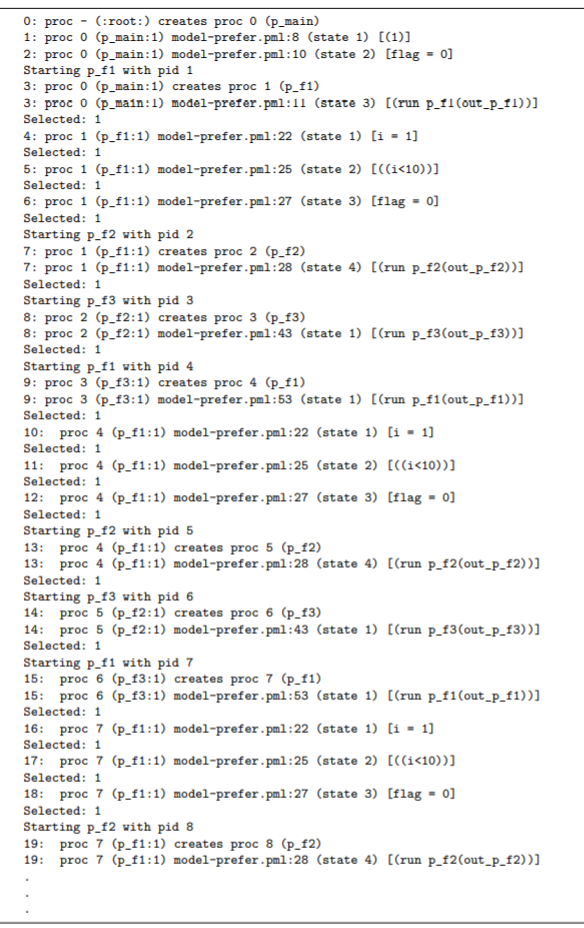
\includegraphics[height=23cm,width=12cm]{l.png}
	\caption{مسیر اجرایی مربوط به کد حاصل از گام سوم}
	\centering
\end{figure}


%\hspace{0.5cm}
%\begin{latin}
%	\begin{lstlisting}
%		0:	proc  - (:root:) creates proc  0 (p_main)
%		1:	proc  0 (p_main:1) model-prefer.pml:8 (state 1)	[(1)]
%		2:	proc  0 (p_main:1) model-prefer.pml:10 (state 2)	[flag = 0]
%		Starting p_f1 with pid 1
%		3:	proc  0 (p_main:1) creates proc  1 (p_f1)
%		3:	proc  0 (p_main:1) model-prefer.pml:11 (state 3)	[(run p_f1(out_p_f1))]
%		Selected: 1
%		4:	proc  1 (p_f1:1) model-prefer.pml:22 (state 1)	[i = 1]
%		Selected: 1
%		5:	proc  1 (p_f1:1) model-prefer.pml:25 (state 2)	[((i<10))]
%		Selected: 1
%		6:	proc  1 (p_f1:1) model-prefer.pml:27 (state 3)	[flag = 0]
%		Selected: 1
%		Starting p_f2 with pid 2
%		7:	proc  1 (p_f1:1) creates proc  2 (p_f2)
%		7:	proc  1 (p_f1:1) model-prefer.pml:28 (state 4)	[(run p_f2(out_p_f2))]
%		Selected: 1
%		Starting p_f3 with pid 3
%		8:	proc  2 (p_f2:1) creates proc  3 (p_f3)
%		8:	proc  2 (p_f2:1) model-prefer.pml:43 (state 1)	[(run p_f3(out_p_f3))]
%		Selected: 1
%		Starting p_f1 with pid 4
%		9:	proc  3 (p_f3:1) creates proc  4 (p_f1)
%		9:	proc  3 (p_f3:1) model-prefer.pml:53 (state 1)	[(run p_f1(out_p_f1))]
%		Selected: 1
%		10:	proc  4 (p_f1:1) model-prefer.pml:22 (state 1)	[i = 1]
%		Selected: 1
%		11:	proc  4 (p_f1:1) model-prefer.pml:25 (state 2)	[((i<10))]
%		Selected: 1
%		12:	proc  4 (p_f1:1) model-prefer.pml:27 (state 3)	[flag = 0]
%		Selected: 1
%		Starting p_f2 with pid 5
%		13:	proc  4 (p_f1:1) creates proc  5 (p_f2)
%		13:	proc  4 (p_f1:1) model-prefer.pml:28 (state 4)	[(run p_f2(out_p_f2))]
%		Selected: 1
%		Starting p_f3 with pid 6
%		14:	proc  5 (p_f2:1) creates proc  6 (p_f3)
%		14:	proc  5 (p_f2:1) model-prefer.pml:43 (state 1)	[(run p_f3(out_p_f3))]
%		Selected: 1
%		Starting p_f1 with pid 7
%		15:	proc  6 (p_f3:1) creates proc  7 (p_f1)
%		15:	proc  6 (p_f3:1) model-prefer.pml:53 (state 1)	[(run p_f1(out_p_f1))]
%		Selected: 1
%		16:	proc  7 (p_f1:1) model-prefer.pml:22 (state 1)	[i = 1]
%		Selected: 1
%		17:	proc  7 (p_f1:1) model-prefer.pml:25 (state 2)	[((i<10))]
%		Selected: 1
%		18:	proc  7 (p_f1:1) model-prefer.pml:27 (state 3)	[flag = 0]
%		Selected: 1
%		Starting p_f2 with pid 8
%		19:	proc  7 (p_f1:1) creates proc  8 (p_f2)
%		19:	proc  7 (p_f1:1) model-prefer.pml:28 (state 4)	[(run p_f2(out_p_f2))]
%		.
%		.
%		.
%	\end{lstlisting}
%\end{latin}
% Chapter 5
\chapter{نتیجه‌گیری}

%%%%%%%%%%%%%%%%%%%%%%%%%%%%%%%
%%%%%%%%%%%%%%%%%%%%%%%%%%%%%%%
\section{پژوهش حاضر}
در این پژوهش سعی بر آن شد تا با تمرکز بر روی مدل‌های با فراخوانی‌های پیچیده‌ی توابع، بهبودی در عملکرد ابزار Modex برای تولید خودکار مدل Promela از کد C صورت گیرد. در این راستا، یک ماژول خودکار توسعه داده‌شد، که فایل Promela تولید شده توسط Modex را به عنوان ورودی دریافت می‎‌کند، و با اعمال اصلاحات بیان شده در فصل پیشین، مدلی بهبودیافته به عنوان خروجی تولید می‌کند.

%%%%%%%%%%%%%%%%%%%%%%%%%%%%%%%
\section{کارهای آتی}
با توجه به بررسی‌هایی که روی کاستی‌های Modex در تولید خودکار کد Promela انجام شد؛ در آینده تلاش برای تعمیم امکان فراخوانی توابع و بهبود مسیر اجرا در هنگام وجود توابع بازگشتی\LTRfootnote{recursive functions} و توابع دارای پارامتر ورودی، صورت خواهد‌گرفت. به علاوه، سعی می‌شود، مطالعات برای اصلاح تبدیل اشاره‌گرها ادامه‌یابد. همچنین ویژگی‌ها\LTRfootnote{properties} و کارایی\LTRfootnote{performance} مدل‌های حاصل از روش‌های پیشنهادی، بررسی خواهدشد.

% Appendices
\appendix
% Appendix 1


% References
\renewcommand{\bibname}{مراجع}
\addcontentsline{toc}{section}{مراجع}

\begin{thebibliography}{99}

\begin{latin}

\baselineskip=.7cm

\bibitem{1}
Spin reference, \textit{https://spinroot.com/spin/Man/README.html}.




\bibitem{2} 
Modex reference, \textit{https://spinroot.com/modex/MANUAL.html}.

\bibitem{3}
K. Havelund and T. Pressburger, \textit{Model checking JAVA programs using
	JAVA PathFinder}, Int. J. Softw. Tools Technol. Transf., vol. 2, no. 4,
pp. 366–381, Apr. 2000.

\bibitem{4} 
Promela reference, \textit{http://spinroot.com/spin/Man/promela.html/}.

\bibitem{5}
B. Vlaovič, A. Vreže and Z. Brezočnik, \textit{Applying Automated Model Extraction for Simulation and Verification of Real-Life SDL Specification With Spin}, in IEEE Access, vol. 5, pp. 5046-5058, 2017, doi: 10.1109/ACCESS.2017.2685238.

\bibitem{6}
K. Jiang, \textit{Model Checking C Programs by Translating C to Promela}, Dissertation, 2009.

\bibitem{7}
H. Mousavi, E. Mahmoudzadeh and A. Ebnenasir, \textit{A Promela Model for Contiki’s Scheduler}, 2020 CSI/CPSSI International Symposium on Real-Time and Embedded Systems and Technologies (RTEST), 2020, pp. 1-10, doi: 10.1109/RTEST49666.2020.9140094.

\end{latin}


\end{thebibliography}

\addcontentsline{toc}{section}{چکیده انگلیسی}
\thispagestyle{empty}

\begin{latin}
\begin{center}

{\Huge Increasing Efficiency in Low-Efficiency Systems}

\vspace{1cm}

{\LARGE{Azin Azadeh}}

\vspace{0.2cm}

{\small azin.azadeh@ec.iut.ac.ir}

\vspace{0.5cm}

March 21, 2015

\vspace{0.5cm}

Department of Electrical and Computer Engineering

\vspace{0.2cm}

Isfahan University of Technology, Isfahan 84156-83111, Iran

\vspace{0.2cm}

Degree: M.Sc. \hspace*{3cm} Language: Farsi

\vspace{1cm}

{\small\textbf{Supervisor: Prof. Bahram Borzou (bahram.borzou@cc.iut.ac.ir)}}
\end{center}
~\vfill



\noindent\textbf{Abstract}

\begin{small}
\baselineskip=0.6cm
In most applications, because of numerous advantages it offers,
digital technology (computer, PLC, microcontroller etc.) is used to
control industrial plants. These types of systems, where the process
under control is continuous-time but the controller is digitally
implemented, are called sampled-data systems. Faults can occur in
sampled-data systems like any other control system. In order to
prevent performance degradation, physical damage or failure, faults
should be promptly detected. In this thesis fault diagnosis in
sampled-data systems is studied. The sampled-data design can be
carried out using direct or indirect design approaches. Direct
design, emphasized in this research, does not involve any
approximations.

Normally, to design a robust fault detection and isolation (FDI)
scheme, a performance index which is a measure of the sensitivity of
the FDI to faults and its robustness to unknown inputs and
disturbances is defined and optimized. Different performance indices
based on norms are considered. Using the direct design
approach and the so-called norm invariant transformation, it is
shown that a sampled-data FDI problem can be converted to an
equivalent discrete-time problem. This will form the foundation of a
unifying framework for optimal sampled-data residual generator
design.

Multirate systems are also abundant in industry. Here, several
methods of residual generation based on multirate sampled data are
developed. The key feature of such residual generators is that they
operate at a fast rate for prompt fault detection. The lifting
technique is used to convert the multirate problem into an
equivalent single-rate discrete-time problem with causality
constraints.

It is generally believed that the optimal multirate design performs
better than the optimal slow-rate and worse than the optimal
fast-rate designs. This conjecture is theoretically proved in this
thesis for general multirate control systems with norms of the
closed-loop system as performance indices. However, it is shown that
the common performance indices in FDI design do not satisfy this
property. To resolve this, an alternative performance index is
defined after formulating the FDI problem as a standard control
problem.

\end{small}

\vspace{0.5 cm}

\noindent \textbf{Key Words}: Fault Detection, Wind Turbine Control, Fault Accomodation, Unknown Input Observers

\end{latin}

%********************************
% Page before last: English Signatures
%********************************
\thispagestyle{empty}
\newgeometry{left=3cm,right=3cm,top=2cm}
\begin{latin}
\begin{center}

\includegraphics[height=3cm]{iut_logo.png}
\vspace{0.4cm}

{\large\textbf{Isfahan University of Technology}}\\

\vspace{0.4cm}
Department of Electrical and Computer Engineering

\vspace{2.5cm}

{\Huge Increasing Efficiency in Low-Efficiency Systems}

\vspace{1.5cm}

{\large
	A Thesis
	
	\vspace{.3cm}
	
	Submitted in partial fulfillment of the requirements
	
	\vspace{.3cm}
	
	for the degree of Master of Science
}

	\vspace{1.5cm}

{\Large
	\textbf{by}
	
	\vspace{.3cm}
	
	\textbf{Azin Azadeh}
}
\end{center}

\vfill

Evaluated and Approved by the Thesis Committee, on March 21, 2015
\vspace{0.5cm}

\begin{enumerate}
\item Bahram Borzou, Prof. (Supervisor)
\vspace{0.5cm}

\item Poorya Parniani, Assoc. Prof. (Advisor)
\vspace{0.5cm}

\item Tahamtan Trabi, Prof. (Examiner)
\vspace{0.5cm}

\item Soraya Sanaei, Assist. Prof (Examiner)
\vspace{0.5cm}

\end{enumerate}

Jamshid Jahangir, Department Graduate Coordinator

\pagebreak
\end{latin}

%***************************
% last page: Blank
%***************************
\thispagestyle{empty}
\mbox{}

% It's finally over. Wasn't that hard, was it?

\end{document}